\documentclass{beamer}
\mode<presentation>
    {
      \usetheme{Madrid}
      \usecolortheme{default}
      \usefonttheme{default}
      \setbeamertemplate{navigation symbols}{}
      \setbeamertemplate{caption}[numbered]
    }
    
\usepackage[english]{babel}
\usepackage[utf8x]{inputenc}
\usepackage{graphicx}
\usepackage{subcaption}


\title[T. e I. de un Motor Gráfico]{Teoría e Implementación de un Motor Gráfico}
\author{Joel Pérez Ferrer}
\institute{Institut de Bruguers}
\date{3/11/2017}

\begin{document}

\begin{frame}
  \titlepage
\end{frame}

\section{Introducción}
\begin{frame}{El Motor Gráfico}
  Un \textbf{motor gráfico} son una serie de rutinas de programación que permiten el diseño, la creación y la representación de entornos interactivos como un videojuego.
  
\begin{figure} [h]
  \centering
  \captionsetup[subfigure]{justification=centering}
  \begin{subfigure}{0.4\textwidth}
    \centering
    
\includegraphics[width=0.8\textwidth]{img/supermario} 
    \caption{\textit{Super Mario Bros.} (1985)}
  \end{subfigure}
  \begin{subfigure}{0.4\textwidth}
    \centering
    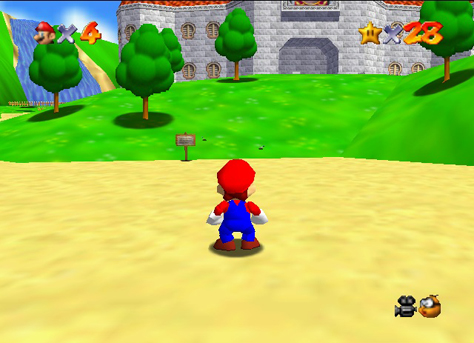
\includegraphics[width=0.8\textwidth]{img/mario64} 
    \caption{\textit{Super Mario 64} (1996)}
  \end{subfigure}
\end{figure}
\end{frame}


\begin{frame}{La Librería Gráfica}
  \begin{itemize}
  \item{La función de la librería gráfica ha ido cambiando a lo largo de los años.}
  \item{La \textbf{librería gráfica} que ha servido de inspiración ha sido OpenGL.}
  \end{itemize}
  \vfill
  \begin{figure}
    \centering
    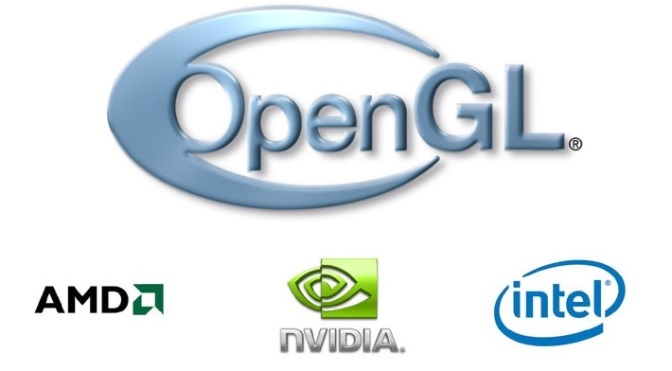
\includegraphics[width=0.5\textwidth]{img/OpenGL-Logo}
  \end{figure}
\end{frame}



\begin{frame}{Objetivos del Treball de Recerca}
  \begin{itemize}
    \item{Factibilidad de desarrollar una librería gráfica}
    \item{Factibilidad de desarrollar un motor gráfico}
    \item{Comprender el funcionamiento de un motor gráfico internamente}
    \item{Familiarizarse con herramientas de expresión científica}
  \end{itemize}
\end{frame}

\begin{frame}{Hipótesis}
  \begin{itemize}
    \item{Hipótesis original:}
  \end{itemize}
  \textit{Los equipos de desarrollo de software deberían de aspirar a ser ellos mismos quienes crean las herramientas que utilizarán para crear el software en sí, En caso de que esta sea una decisión no rentable, su máxima prioridad debería de ser entender cómo funcionan las herramientas que utilizarán.}
\end{frame}

\begin{frame}{Metodología}
  Un resultado final, muchas formas de llegar a él.
  \vfill
  \begin{figure} [h]
    \centering
    
\includegraphics[width=0.3\textwidth]{img/rubik}
  \end{figure}
\end{frame}

\begin{frame}{Herramientas: Programación}
  \begin{itemize}
  \item{Lenguaje de Programación: C++ $\rightarrow$ \textbf{C/C++} $\rightarrow$ C++}
  \item{Compilador: \textbf{GNU Compiler Collection (GCC)}, MinGW GCC}
  \item{Editor de texto: \textbf{GNU Emacs}}
  \item{IDE: \textbf{Code::Blocks}}
  \item{Depurador: \textbf{GNU Project Debugger (GDB)}, interfaz GDB de Code::Blocks}
  \item{Sistema Operativo: \textbf{GNU/Linux}, MS Windows y macOS}
  \item{Gestor de código: \textbf{git} (\textit{Github})}
  \end{itemize}
  \begin{figure} [h]
    \centering
    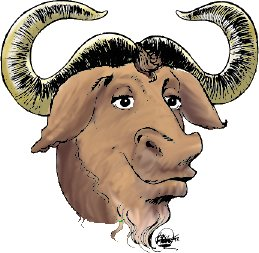
\includegraphics[width=0.2\textwidth]{img/reiss-head}
  \end{figure}
\end{frame}

\begin{frame}{Herramientas: Documentación}
  Tanto para el documento escrito como para en la presentación se han usado \textbf{las mismas herramientas}.
  \begin{itemize}
  \item{Lenguaje de Programación: \textrm{\LaTeX}}
  \item{Compilador: \textrm{\TeX  Live}}
  \item{Editor de texto: GNU Emacs}
  \item{Diagramas: Ti\textit{k}Z and PGF y GeoGebra}
  \end{itemize}
\end{frame}

\begin{frame}{Espacio local}
\end{frame}
\begin{frame}{Espacio global}
\end{frame}
\begin{frame}{Espacio de vista}
\end{frame}
\begin{frame}{Espacio NDC}
\end{frame}
\begin{frame}{Espacio de ventana}
\end{frame}

\section{Conclusión}
\begin{frame}{Ajustes del método}
\end{frame}
\begin{frame}{Revisión de la hipótesis}
\end{frame}
\begin{frame}{Preguntas}
\end{frame}
\begin{frame}{Valoración personal}
\end{frame}

\end{document}
